\chapter{Two-team Markov game supplementary materials} \label{ch:ch7_appendix}
\section{Training parameters}
\label{app:train_param}
The learning parameters of the three methods were determined by default configurations provided by their different authors.
They are the same as the ones used in QVMix implementation \citep{leroy2020qvmix}.
We hereafter provide a description of some of these training parameters.

Individual networks are 64 cells GRU enclosed with fully connected layers (see Fig \ref{fig:indivQ}).
The mixer network is the same as in \citep{Rashid2018} with an embedded size of 32.
The individual and mixer networks are the same for the three methods.
We used the default parameters of MAVEN policy networks provided by \citep{Mahajan2019MAVEN:Exploration}.
For QVMix, the $V$ network is a copy of the QMIX network with only one output for each $V$ network.

For each learning scenario, networks are updated regardless of how episodes have been generated.
Networks are updated from a replay buffer that collects the $5000$ latest played episodes and $32$ of them are sampled from it to update the network.
The network update is performed every eight episodes in the $3m$ map and every episode in the $3s5z$ map.
The difference is justified by the desire to increase the number of network updates for $3s5$ to improve performances, especially against the heuristic.
The epsilon greedy exploration starts with an epsilon equal to $1$ decreasing linearly to $0.05$ during $2$ million timesteps.
This is perhaps the main difference between the provided parameters, which decrease the epsilon only during $0.5$ million timesteps.
The discount factor is $\gamma = 0.99$ and the learning rate is $0.0005$.
Target networks are updated every $200$ episode.
We refer the reader to \citep{Mahajan2019MAVEN:Exploration} for further parameter definitions for MAVEN optimisation.

\section{Training time}
\label{app:train_time}

\begin{figure}[ht]
    \centering
    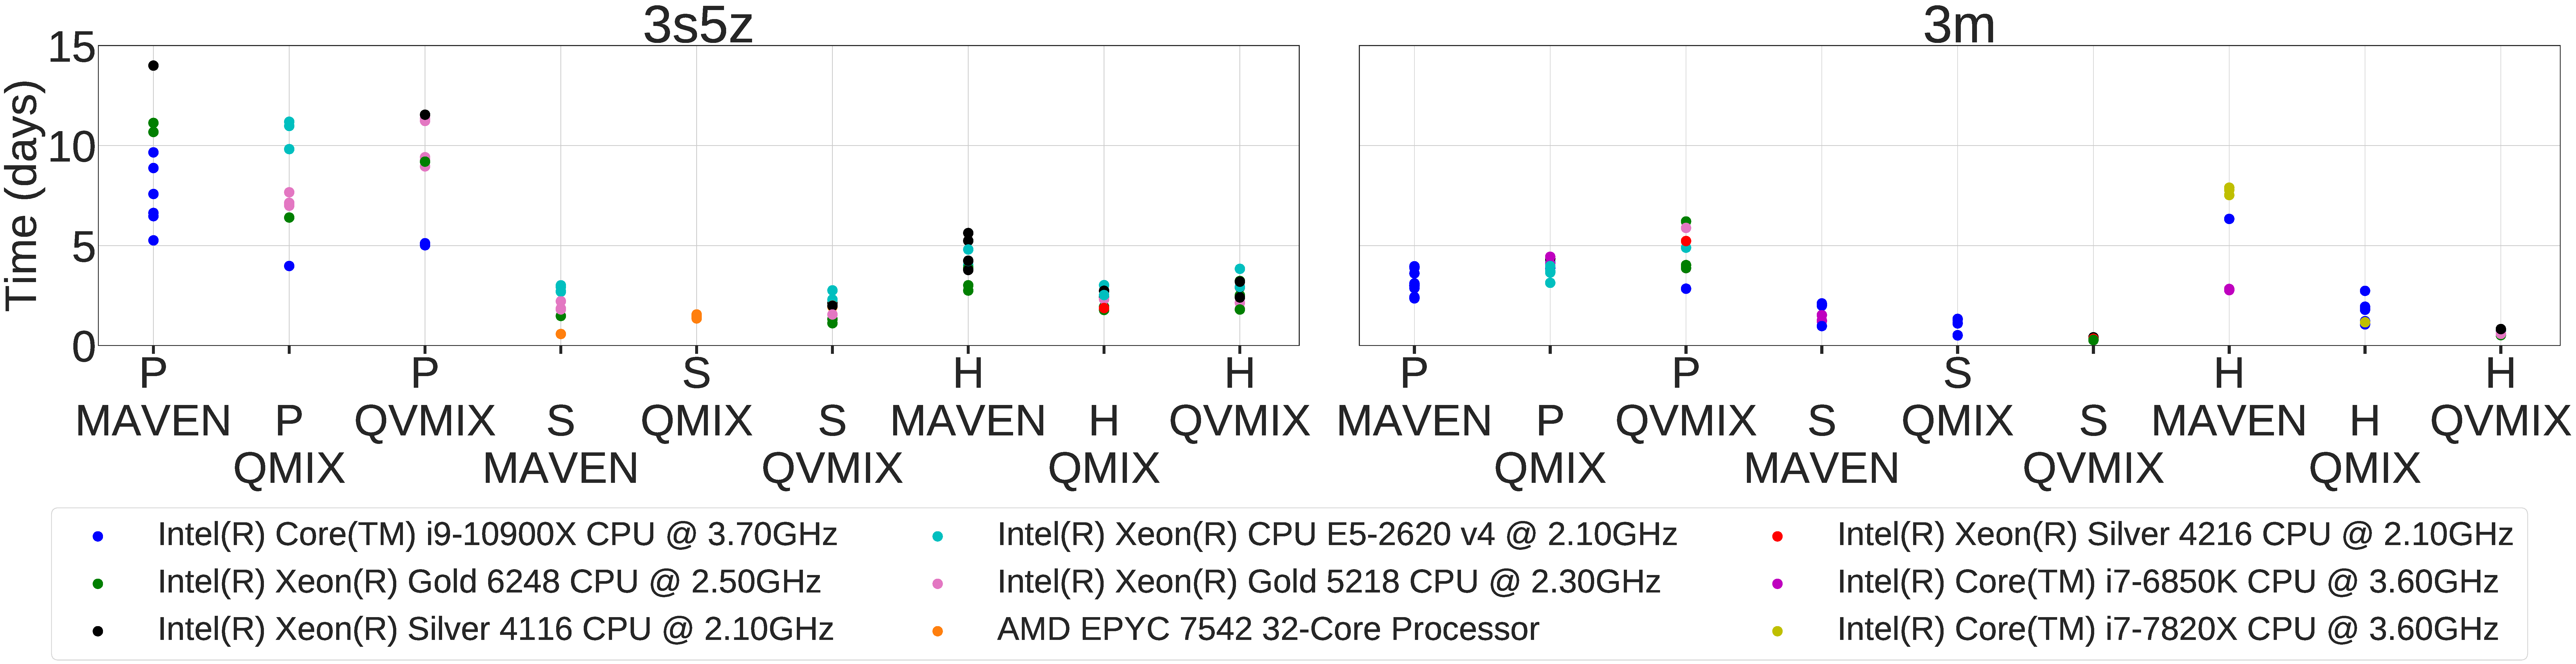
\includegraphics[width=\textwidth]{tex_thesis/figures/ch7/training_time.pdf}
    \caption{Training duration, in days, for the different learning scenarios tested in this paper.
    The different colours represent the different CPUs that have been used to perform the experiments.}
    \label{fig:training_time}
\end{figure}

Experiments were performed with CPUs only because small recurrent neural networks do not arguably benefit from GPU.
We had access to several types of computers, with different numbers of CPUs accessible at the same time.
Training times for each experiment performed are presented in Figure \ref{fig:training_time}.
With all these different hardware configurations, it is not possible to rigorously compare the times of the experiments.
However, it is possible to present the time complexity.
As explained in Section \ref{sec:experiments}, training in self-play requires five times fewer environment timesteps than training within a population but also five times fewer network updates.
Furthermore, when training a population, networks are updated sequentially, which also increases the time.
Finally, SC2 processes are prone to errors and, therefore, sometimes need to be restarted.
As the actions of all agents in the different running environments are performed simultaneously, these restarts are time-consuming operations as the processes have to wait for the faulty one.
